\documentclass[parskip]{cs4rep}

\usepackage{hyperref}
\usepackage{todonotes}
\usepackage{natbib}
\usepackage{subcaption}

\begin{document}

\title{Clustering and Visualisation\\ of DNA Sequencing Data}

\author{Saulius Lukauskas}

\degree{Artificial Intelligence}
\project{Undergraduate Dissertation}

\date{\today}

\abstract{
\todo{Need an abstract}
}

\maketitle

%\section*{Acknowledgements}
%Acknowledgements go here.

\tableofcontents

%\pagenumbering{arabic}


\chapter{Background and Introduction}

The complete set of information required to create and maintain cells of a
living organism is contained in the genome of the organism. In humans, this
information is encoded in a long chain of nucleotides within the DNA molecules
in 23 different chromosomes located in the nucleus of every cell as well as in
a small segment of DNA located within the mitochondrion of the cell.  
These chains of nucleotides can be sequenced by determining the order of appearance
of the four bases within the genome: adenine (often abbreviated as simply "A"), cytosine (abbreviated as C),
guanine (G) or thymine (T).
The sequence of these nucleobases is commonly referred to as the DNA Sequence. 

\section{Structure of  DNA}
Generally DNA molecules are observed in pairs of two tightly connected
molecules, rather than as a single molecule. These molecules are known as
strands and are held together by the bonds between the nucleobases: guanine is
known to form a bond with cytosine, whereas adenine forms a bond with thymine.
Since each kind of nucleobase can form a bond with only one other kind of
nucleobase, both of the DNA strands contain enough information to recreate the
other on its own. This redundancy is required for DNA replication process. 

Because of this redundancy, the sequences on complimentary strands are often considered at the
same time as sequences of base pairs, rather than sequences of nucleotides. The
human sex cells are known to contain around three billion such base pairs.

\subsection{Histones}
\todo{Fill me in}
\subsection{Transcription and Splicing}
\todo{Need to explain here what are transcription start sites, exons and why they are important}

\section{Next-Generation Sequencing}
The Human Genome Project was the research project that has sequenced all
three billion of these base pairs for the first time. The project was estimated
to cost 3 billion dollars for American tax payers and last 15 years, but has ended up
costing a bit less than that - \$2.7 billion and was completed in 13
years\footnote{See \url{http://www.genome.gov/11006943} and
    \url{http://www.ornl.gov/sci/techresources/Human_Genome/project/about.shtml}
    for more information}. 
    
 Since then, a variety of DNA sequencing methods were
developed that reduce both the time and cost required to perform sequencing
significantly\citep{Shendure:2008uc,Liu:2012ve}. New technology and reduced
costs of DNA Sequencing has made it more accessible and allowed
development of new genome-scale analysis methods such as ChIP-Sequencing
(ChIP-Seq).

\section{ChIP Sequencing}

\chapter{Motivation}


\section{Previous art}

\todo{Mention the two major papers in the game}

\chapter{Methods}
\section{Dynamic Time Warping}
Underneath the methods used in this project, lies the Dynamic Time Warping (DTW) algorithm. This algorithm was initially developed in the speech recognition community in order to allow accurate comparisons between words spoken with tempo variations. 
This comparison is achieved by warping the time axis nonlinearly. That is, the axis is stretched or compressed arbitrarily as to minimise the total distance between the points aligned to each other. For example see figure \ref{fig:DTW:alignments}, there two sequences are aligned to each other. Those two sequences are sine and cosine over the range $[-pi; pi)$ therefore we are confident that they share similar patterns, just at different locations.

In figure \ref{fig:DTW:euclidean_alignment}, each point on the sequence A is aligned to corresponding point on the sequence B. If we were to sum the distances between aligned points, we would get the Euclidean distance between these two sequences. We can see that the alignment is not very good as the highest point on the first sequence is mapped to a mid-point of the second.

The mapping seen in \ref{fig:DTW:dtw_alignment} is completely different. The highest points are now mapped to each other, so are the other points that are in the patterns existing in both of the sequences. If we were to calculate the differences between the mapped points again, we would see that the resulting distance is much smaller than Euclidean one.

\begin{figure}[t,b]
   \centering
   \begin{subfigure}[b]{0.4\textwidth}
       \centering
       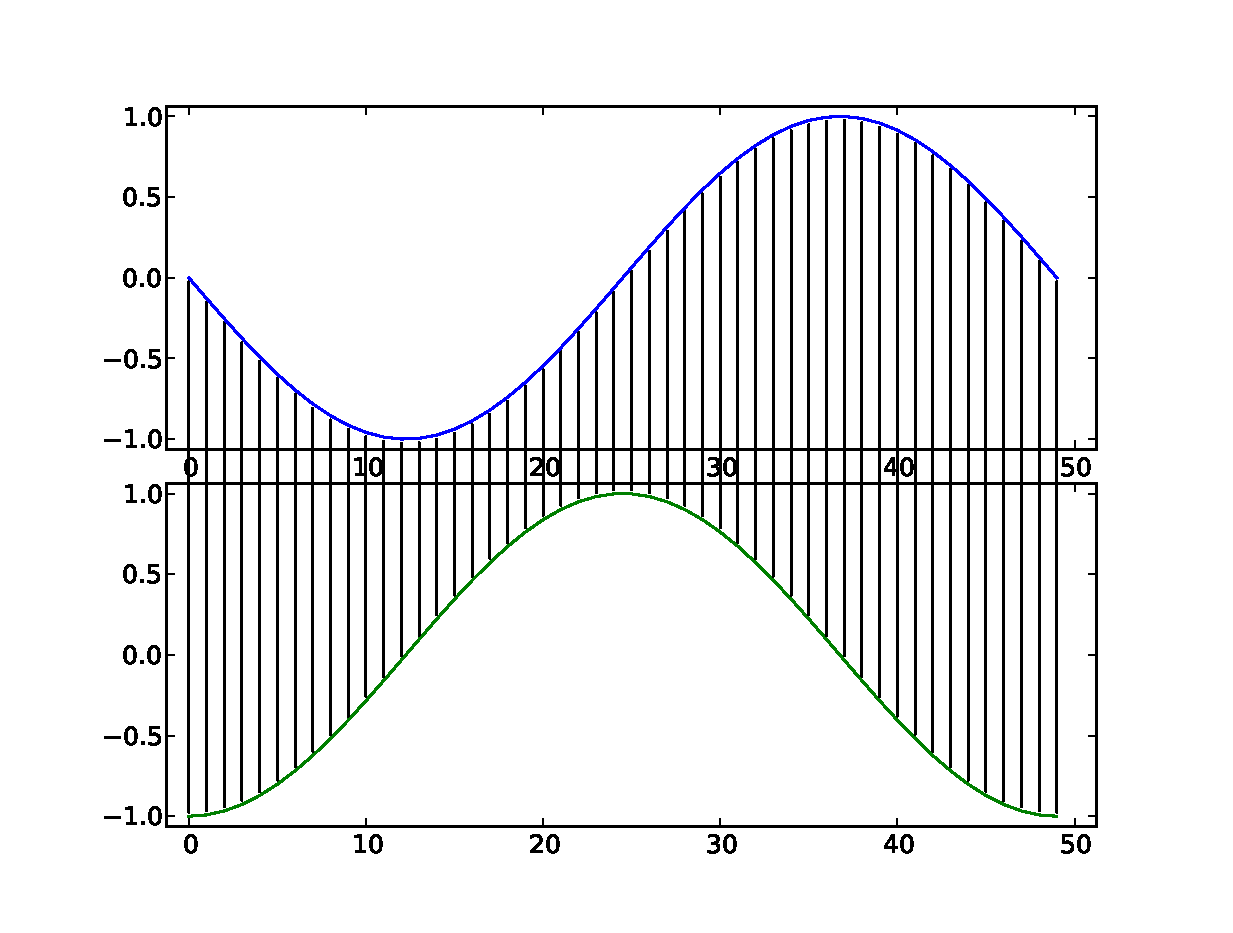
\includegraphics[width=\textwidth]{figures/DTW/sin-cos-no-dtw.eps}
       \caption{Euclidean alignment}
       \label{fig:DTW:euclidean_alignment}
   \end{subfigure}
   ~
   \begin{subfigure}[b]{0.4\textwidth}
       \centering
       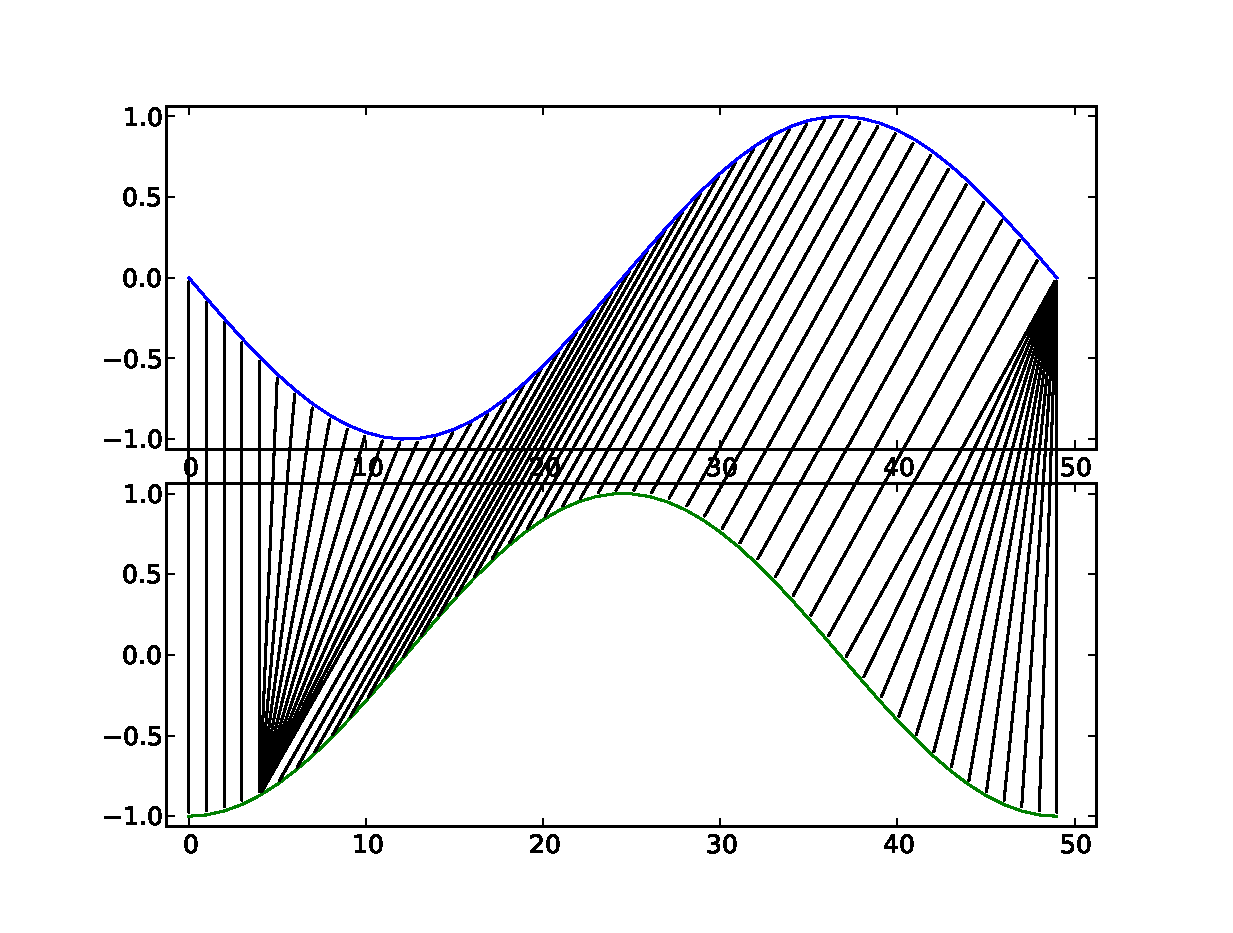
\includegraphics[width=\textwidth]{figures/DTW/sin-cos-dtw.eps}
       \caption{DTW alignment}
       \label{fig:DTW:dtw_alignment}
   \end{subfigure}
   
   \caption{Two sequences aligned to each other. Figure \ref{fig:DTW:euclidean_alignment} maps each point on sequence A to a point on sequence B directly, resulting in an Euclidean distance measure, whereas figure \ref{fig:DTW:dtw_alignment} uses Dynamic Time Warping algorithm to find a better mapping between the points}
   \label{fig:DTW:alignments}
\end{figure}

\missingfigure{Streching-compressing axis}

\subsection{Constrained DTW}
\subsection{Constant-Penalty DTW}
\section{Agglomerative clustering}
\todo{Make sure to write about: 1) Triangle inequality and stuff, 2) complete linkage}
\section{Prototyping and Visualisation}
\section{Biologically Relevant Heuristics}
\todo{Write about antisense regions correction}

\chapter{Implementation Details}
\todo{Mention and cite all the libraries DTW builds on}

\section{File formats}
\subsection{BAM}
\subsection{BED}

\section{Time Complexity}
\subsection{Native-C Modules}
\subsection{Parallel processing}
\todo{Write about how expensive DTW is, write about what a pain is to do multiprocessing it in Python}

\chapter{Results}

\chapter{Conclusions and Contributions}

\bibliographystyle{alpha}
\bibliography{papers2}

\appendix
\todo{Include both papers}

\end{document}
